\newpage
\hypertarget{body-content}{}
\hypertarget{introduction-to-data-structures-and-algorithms}{%
	\mysection{Introduction to Data Structures and
		Algorithms}\label{introduction-to-data-structures-and-algorithms}}

Data Structure is a way of collecting and organising data in such a way
that we can perform operations on these data in an effective way. Data
Structures is about rendering data elements in terms of some
relationship, for better organization and storage. For example, we have
some data which has, player's \textbf{name} "Virat" and \textbf{age} 26.
Here "Virat" is of \textbf{String} data type and 26 is of
\textbf{integer} data type.

We can organize this data as a record like \textbf{Player} record, which
will have both player's name and age in it. Now we can collect and store
player's records in a file or database as a data structure. \textbf{For
example}: "Dhoni" 30, "Gambhir" 31, "Sehwag" 33

If you are aware of Object Oriented programming concepts, then a
\texttt{class} also does the same thing, it collects different type of
data under one single entity. The only difference being, data structures
provides for techniques to access and manipulate data efficiently.

In simple language, Data Structures are structures programmed to store
ordered data, so that various operations can be performed on it easily.
It represents the knowledge of data to be organized in memory. It should
be designed and implemented in such a way that it reduces the complexity
and increases the efficiency.

\begin{center}\rule{0.5\linewidth}{0.5pt}\end{center}

\hypertarget{basic-types-of-data-structures}{%
	\mysubsection{Basic types of Data
		Structures}\label{basic-types-of-data-structures}}

As we have discussed above, anything that can store data can be called
as a data structure, hence Integer, Float, Boolean, Char etc, all are
data structures. They are known as \textbf{Primitive Data Structures}.\\

Then we also have some complex Data Structures, which are used to store
large and connected data. Some example of \textbf{Abstract Data
Structure} are :

\begin{itemize}
	\tightlist
	\item
	      Linked List
	\item
	      Tree
	\item
	      Graph
	\item
	      Stack, Queue etc.
\end{itemize}

All these data structures allow us to perform different operations on
data. We select these data structures based on which type of operation
is required. We will look into these data structures in more details in
our later lessons.

\begin{figure}
    \centering
    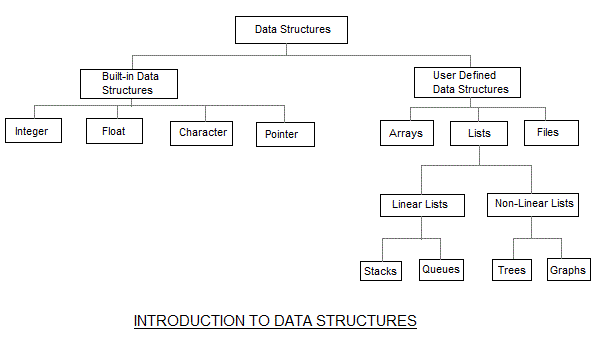
\includegraphics[scale=.5]{images/introduction-to-data-structures.png}
    \caption{Caption}
    \label{fig:my_label}
\end{figure}


\hfill\break

The data structures can also be classified on the basis of the following
characteristics:

\begin{table}
\begin{tabular}{|p{.20\textwidth}|p{.8\textwidth}|}
	\hline
	\textbf{Characteristic}   & \textbf{Description}\\                    
	\hline
	Linear          & In Linear data structures,the data items are arranged in a linear sequence. Example: \textbf{Array}\\
	\hline
	Non-Linear      & In Non-Linear data structures,the data items are not in sequence. Example: \textbf{Tree}, \textbf{Graph}\\
	\hline
	Homogeneous     & In homogeneous data structures,all the elements are of same type. Example: \textbf{Array}\\
	\hline
	Non-Homogeneous & In Non-Homogeneous data structure, the elements may or may not be of the same type. Example: \textbf{Structures}\\
	\hline
	Static          & Static data structures are those whose sizes and structures associated memory locations are fixed, at compile time. Example:\textbf{Array}\\
	\hline
	Dynamic         & Dynamic structures are those which expands or shrinks depending upon the program need and its execution. Also, their associated memory locations changes. Example: \textbf{Linked List created using pointers}\\
	\hline
\end{tabular}
\end{table}
\begin{center}\rule{0.5\linewidth}{0.5pt}\end{center}

\hypertarget{what-is-an-algorithm}{%
	\mysubsection{What is an Algorithm ?}\label{what-is-an-algorithm}}

An algorithm is a finite set of instructions or logic, written in order, to accomplish a certain predefined task. Algorithm is not the complete code or program, it is just the core logic(solution) of a problem, which can be expressed either as an informal high level description as \textbf{pseudocode} or using a \textbf{flowchart}.\\

Every Algorithm must satisfy the following properties:

\begin{enumerate}
	\tightlist
	\item
	      \textbf{Input}- There should be 0 or more inputs supplied externally
	      to the algorithm.
	\item
	      \textbf{Output}- There should be atleast 1 output obtained.
	\item
	      \textbf{Definiteness}- Every step of the algorithm should be clear and
	      well defined.
	\item
	      \textbf{Finiteness}- The algorithm should have finite number of steps.
	\item
	      \textbf{Correctness}- Every step of the algorithm must generate a
	      correct output.
\end{enumerate}

An algorithm is said to be efficient and fast, if it takes less time to execute and consumes less memory space. The performance of an algorithm is measured on the basis of following properties :

\begin{enumerate}
	\tightlist
	\item
	      Time Complexity
	\item
	      Space Complexity
\end{enumerate}

\begin{center}\rule{0.5\linewidth}{0.5pt}\end{center}

\hypertarget{space-complexity}{%
	\mysubsection{Space Complexity}\label{space-complexity}}

Its the amount of memory space required by the algorithm, during the course of its execution. Space complexity must be taken seriously for multi-user systems and in situations where limited memory is available.\\

An algorithm generally requires space for following components :

\begin{itemize}
	\tightlist
	\item
	      \textbf{Instruction Space:} Its the space required to store the
	      executable version of the program. This space is fixed, but varies
	      depending upon the number of lines of code in the program.
	\item
	      \textbf{Data Space:} Its the space required to store all the constants
	      and variables(including temporary variables) value.
	\item
	      \textbf{Environment Space:} Its the space required to store the
	      environment information needed to resume the suspended function.
\end{itemize}


\hypertarget{time-complexity}{%
	\mysubsection{Time Complexity}\label{time-complexity}}

Time Complexity is a way to represent the amount of time required by the program to run till its completion. It's generally a good practice to try to keep the time required minimum, so that our algorithm completes it's execution in the minimum time possible. 

\hypertarget{body-content}{}
\hypertarget{space-complexity-of-algorithms}{%
\section{Space Complexity of
Algorithms}\label{space-complexity-of-algorithms}}

Whenever a solution to a problem is written some memory is required to
complete. For any algorithm memory may be used for the following:

\begin{enumerate}
\tightlist
\item
  Variables (This include the constant values, temporary values)
\item
  Program Instruction
\item
  Execution
\end{enumerate}

\begin{quote}
\emph{\textbf{Space complexity} is the amount of memory used by the
algorithm (including the input values to the algorithm) to execute and
produce the result.}
\end{quote}

Sometime \textbf{Auxiliary Space} is confused with Space Complexity. But
Auxiliary Space is the extra space or the temporary space used by the
algorithm during it's execution.

\textbf{Space Complexity} = \textbf{Auxiliary Space + Input space}

\begin{center}\rule{0.5\linewidth}{0.5pt}\end{center}

\hypertarget{memory-usage-while-execution}{%
\mysubsection{Memory Usage while Execution}\label{memory-usage-while-execution}}

While executing, algorithm uses memory space for three reasons:

\begin{enumerate}
\item
  \textbf{Instruction Space}

  It's the amount of memory used to save the compiled version of
  instructions.
\item
  \textbf{Environmental Stack}

  Sometimes an algorithm(function) may be called inside another
  algorithm(function). In such a situation, the current variables are
  pushed onto the system stack, where they wait for further execution
  and then the call to the inside algorithm(function) is made.

  For example, If a function \texttt{A()} calls function \texttt{B()}
  inside it, then all th variables of the function \texttt{A()} will get
  stored on the system stack temporarily, while the function
  \texttt{B()} is called and executed inside the funciton \texttt{A()}.
\item
  \textbf{Data Space}

  Amount of space used by the variables and constants.
\end{enumerate}

But while calculating the \textbf{Space Complexity} of any algorithm, we usually consider only \textbf{Data Space} and we neglect the \textbf{Instruction Space} and \textbf{Environmental Stack}.

\begin{center}\rule{0.5\linewidth}{0.5pt}\end{center}

\hypertarget{calculating-the-space-complexity}{%
\mysubsection{Calculating the Space
Complexity}\label{calculating-the-space-complexity}}

For calculating the space complexity, we need to know the value of
memory used by different type of datatype variables, which generally
varies for different operating systems, but the method for calculating
the space complexity remains the same.

\begin{longtable}[]{@{}ll@{}}
\toprule
Type & Size\tabularnewline
\midrule
\endhead
bool, char, unsigned char, signed char, \_\_int8 & 1 byte\tabularnewline
\_\_int16, short, unsigned short, wchar\_t, \_\_wchar\_t & 2
bytes\tabularnewline
float, \_\_int32, int, unsigned int, long, unsigned long & 4
bytes\tabularnewline
double, \_\_int64, long double, long long & 8 bytes\tabularnewline
\bottomrule
\end{longtable}

\hfill\break

Now let's learn how to compute space complexity by taking a few
examples:

\begin{minted}[]
{
    int z = a + b + c;
    return(z);
}
\end{minted}

In the above expression, variables \texttt{a}, \texttt{b}, \texttt{c}
and \texttt{z} are all integer types, hence they will take up 4 bytes
each, so total memory requirement will be
\texttt{(4(4)\ +\ 4)\ =\ 20\ bytes}, this additional 4 bytes is for
\textbf{return value}. And because this space requirement is fixed for
the above example, hence it is called \textbf{Constant Space
Complexity}.

Let's have another example, this time a bit complex one,

\begin{minted}[]
// n is the length of array a[]
int sum(int a[], int n)
{
    int x = 0;     // 4 bytes for x
    for(int i = 0; i < n; i++)  // 4 bytes for i
    {    
        x  = x + a[i];     
    }
    return(x);
}
\end{minted}

\begin{itemize}
\tightlist
\item
  In the above code, \texttt{4*n} bytes of space is required for the
  array \texttt{a{[}{]}} elements.
\item
  4 bytes each for \texttt{x}, \texttt{n}, \texttt{i} and the return
  value.
\end{itemize}

Hence the total memory requirement will be \texttt{(4n\ +\ 12)}, which is increasing linearly with the increase in the input value \texttt{n}, hence it is called as \textbf{Linear Space Complexity.}

Similarly, we can have quadratic and other complex space complexity as well, as the complexity of an algorithm increases.

But we should always focus on writing algorithm code in such a way that we keep the space complexity \textbf{minimum}.



